\documentclass[11pt,letterpaper]{article}
\usepackage[provide=*,spanish]{babel}
\usepackage[utf8]{inputenc}
\usepackage[T1]{fontenc}
\usepackage{lmodern}
\usepackage{geometry,graphicx,tabularx,array,booktabs,float}
\usepackage{enumitem}
\usepackage[hidelinks]{hyperref}
\usepackage{fancyhdr}
\geometry{margin=2.1cm}
\setlength{\parindent}{0pt}
\setlength{\parskip}{6pt}
\renewcommand{\arraystretch}{1.18}
\pagestyle{fancy}
\setlength{\headheight}{14pt}
\fancyhf{}
\fancyhead[L]{NOVATECH  |  Taller de Desarrollo 3}
\fancyhead[R]{Fernando Aguilar López}
\fancyfoot[C]{\thepage}
\setlist[itemize]{leftmargin=1.4em,topsep=2pt,itemsep=2pt}
\begin{document}

\begin{titlepage}
\centering
\vspace*{2.5cm}
{\Large Universidad Autónoma de Chiapas\par}
\vspace{.35cm}
{\large Licenciatura en Ingeniería en Desarrollo y Tecnologías de Software\par}
\vspace{2cm}
{\Huge\bfseries NOVATECH\par}
\vspace{.5cm}
{\LARGE Documentación de la entrega del sábado\par}
\vspace{1cm}
{\large Registro, autorización de acceso y consulta de productos\par}
\vfill
{\large Alumno: Aguilar López Fernando\par}
{\large Asignatura: Taller de Desarrollo 3\par}
{\large Tuxtla Gutiérrez, Chiapas\par}
{\large 26 de septiembre de 2026\par}
\end{titlepage}

\section*{Resumen de la entrega}
NOVATECH es un prototipo de tienda de laptops con frontend React y Vite, backend Node.js y Express, y base de datos PostgreSQL. Esta entrega demuestra el registro de una cuenta, el bloqueo de acceso mientras está pendiente, la aprobación y asignación del rol Pedidos por el súper administrador, y la consulta de dos productos con imagen, descripción y precio. Las imágenes son archivos del frontend; PostgreSQL almacena sus rutas.

El alcance probado para el sábado se centra en autenticación, control de acceso y catálogo de consulta. La actividad completa también solicita CRUD de tres entidades, módulos adicionales, aprobación de ventas y captcha; esas funciones no se presentan aquí como terminadas.

\section{Objetivo y alcance}
El objetivo de esta etapa es verificar que una persona nueva no entre al sistema hasta recibir autorización, y que al ser aprobada con el rol Pedidos consulte únicamente el catálogo disponible. El administrador decide aprobar o rechazar la solicitud y elige el rol. Se registraron dos laptops de ejemplo.

\begin{tabularx}{\textwidth}{>{\raggedright\arraybackslash}p{4.0cm}X}
\toprule
\textbf{Componente} & \textbf{Función observada}\\ \midrule
Frontend & Formulario de registro e inicio de sesión; panel del súper administrador; catálogo del rol Pedidos.\\
Backend & API HTTP para autenticación, solicitudes de acceso y consulta de productos.\\
PostgreSQL & Persistencia de usuarios, decisiones de acceso y datos de los productos.\\
Archivos de imagen & \texttt{frontend/public/productos/}; la tabla de productos guarda \texttt{imagen\_url}.\\
\bottomrule
\end{tabularx}

\section{Arquitectura del sistema}
El navegador ejecuta React y llama a funciones aisladas en \texttt{frontend/src/services/api.js}. Estas envían peticiones HTTP a Express en el puerto 4000. El backend aplica el control de acceso y consulta PostgreSQL. Vite sirve las imágenes estáticas del directorio \texttt{public/productos} en el puerto 5173.

\begin{center}
\fbox{React y Vite $\longrightarrow$ servicio API $\longrightarrow$ Express $\longrightarrow$ PostgreSQL}\\[5pt]
\fbox{\texttt{public/productos/*.png} $\longrightarrow$ navegador mediante Vite}
\end{center}

La consigna solicita separación en dominio, aplicación, puertos, adaptadores e interfaces. El diagrama anterior expresa las conexiones comprobadas en esta etapa; la organización interna del backend debe verificarse directamente en el repositorio antes de afirmar que toda la arquitectura hexagonal está completa.

\section{Endpoints utilizados en esta etapa}
La URL base configurada por el frontend es \texttt{http://localhost:4000/api}. La siguiente lista procede del servicio \texttt{api.js} usado para las pantallas probadas.

\begin{tabularx}{\textwidth}{>{\ttfamily\small}p{1.45cm}>{\ttfamily\small}p{6.1cm}X}
\toprule
\textbf{Método} & \textbf{Ruta} & \textbf{Uso}\\ \midrule
POST & /auth/registro & Registrar cuenta pendiente.\\
POST & /auth/login & Iniciar sesión y recibir la sesión autorizada.\\
GET & /admin/solicitudes & Consultar cuentas pendientes (súper admin).\\
PATCH & /admin/usuarios/:id/acceso & Aprobar o rechazar y asignar rol.\\
GET & /productos & Consultar catálogo con rol Pedidos.\\
\bottomrule
\end{tabularx}

Las rutas protegidas reciben el token en la cabecera \texttt{Authorization: Bearer <token>}. Esta tabla documenta las rutas utilizadas; no sustituye la especificación del CRUD completo solicitado para la fase posterior.

\section{Productos y almacenamiento de imágenes}
\begin{tabularx}{\textwidth}{>{\raggedright\arraybackslash}p{3.5cm}X>{\raggedleft\arraybackslash}p{2.6cm}}
\toprule
\textbf{Producto} & \textbf{Descripción y ruta de imagen} & \textbf{Precio MXN}\\ \midrule
Laptop para estudio & Clases, tareas y navegación diaria. \texttt{/productos/laptop-estudio.png} & \$12,999.00\\
Laptop gamer & Videojuegos y aplicaciones exigentes. \texttt{/productos/laptop-gamer.png} & \$21,999.00\\
\bottomrule
\end{tabularx}

La consulta a PostgreSQL confirmó las dos rutas \texttt{.png}. Los archivos se guardaron en \nolinkurl{frontend/public/productos}; por ello las fotos no se almacenan como datos binarios en la base.

\clearpage
\section{Pruebas y evidencias}
La secuencia se probó desde el navegador: registrar una cuenta nueva, intentar entrar antes de la aprobación, verla en el panel del súper administrador, aprobarla con el rol Pedidos y entrar nuevamente para ver el catálogo. En las capturas, la cuenta de prueba figura como \texttt{cliente2@tienda.local}.

\begin{figure}[H]\centering

\includegraphics[width=.78\textwidth]{imagenes/01-registro-pendiente.png}
\caption{El registro genera una solicitud pendiente.}
\end{figure}
\begin{figure}[H]\centering
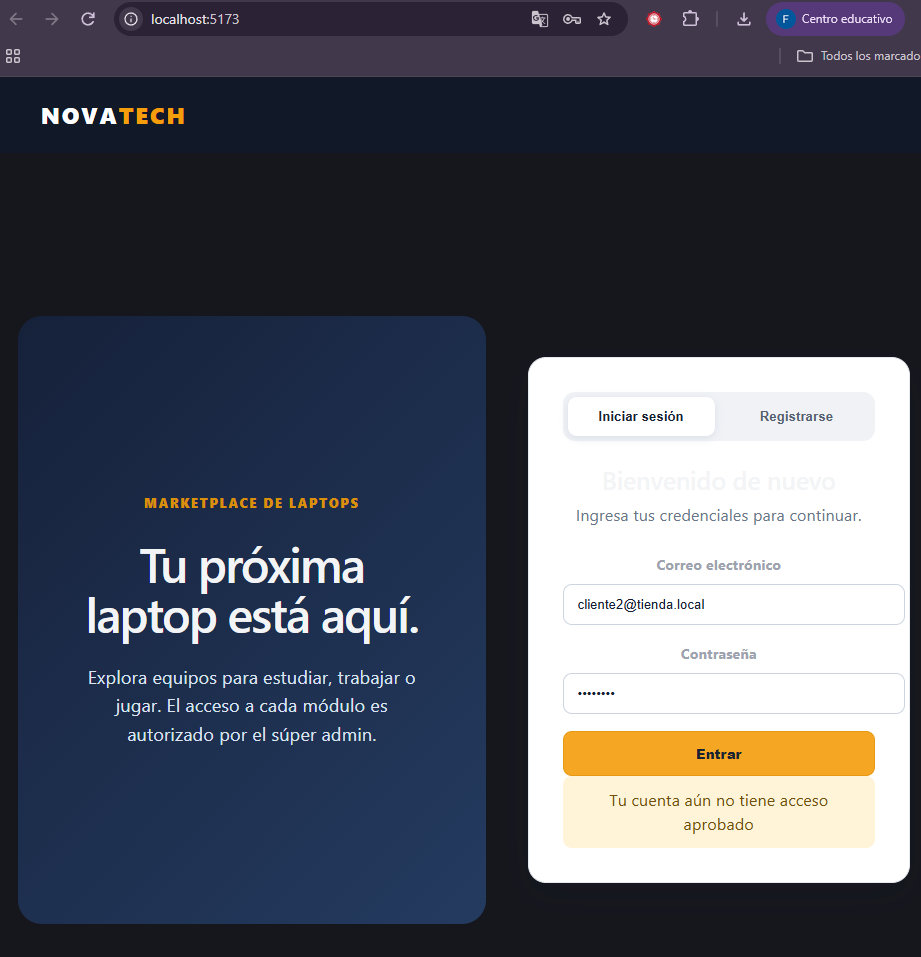
\includegraphics[width=.78\textwidth]{imagenes/02-acceso-pendiente.png}
\caption{El inicio de sesión queda bloqueado antes de la autorización.}
\end{figure}

\clearpage
\begin{figure}[H]\centering
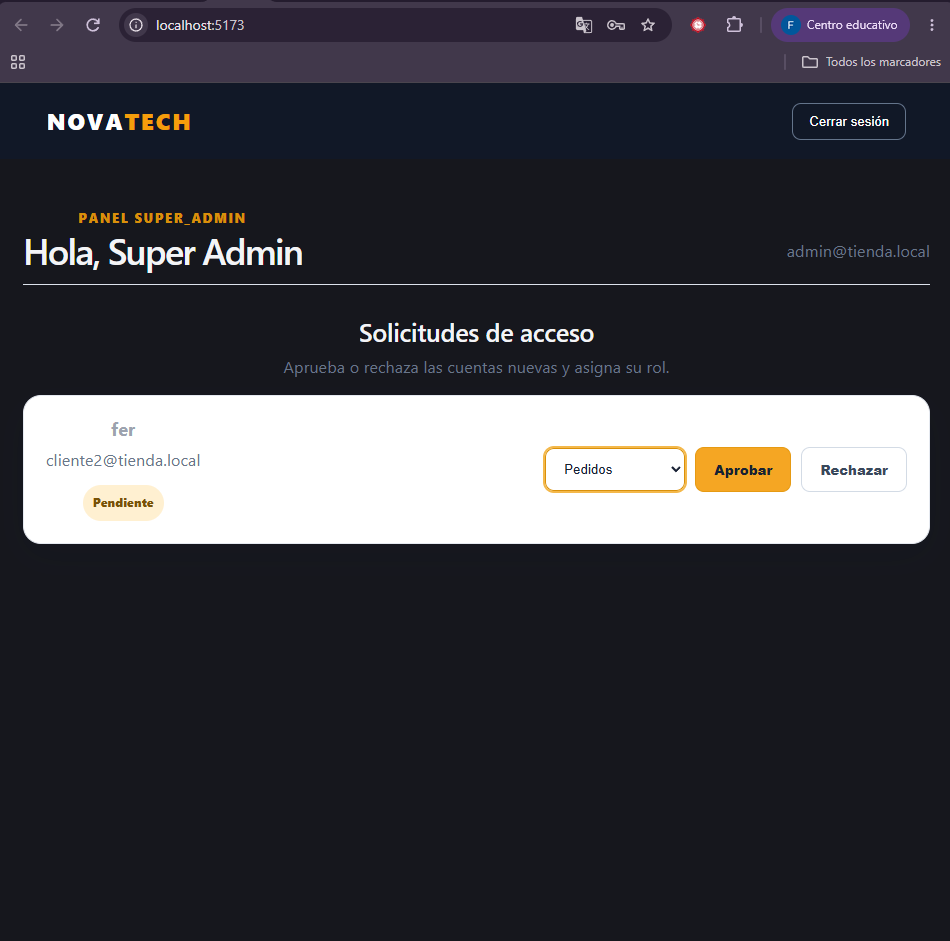
\includegraphics[width=.84\textwidth]{imagenes/03-solicitud-admin.png}
\caption{El súper administrador recibe la solicitud y selecciona Pedidos.}
\end{figure}
\begin{figure}[H]\centering
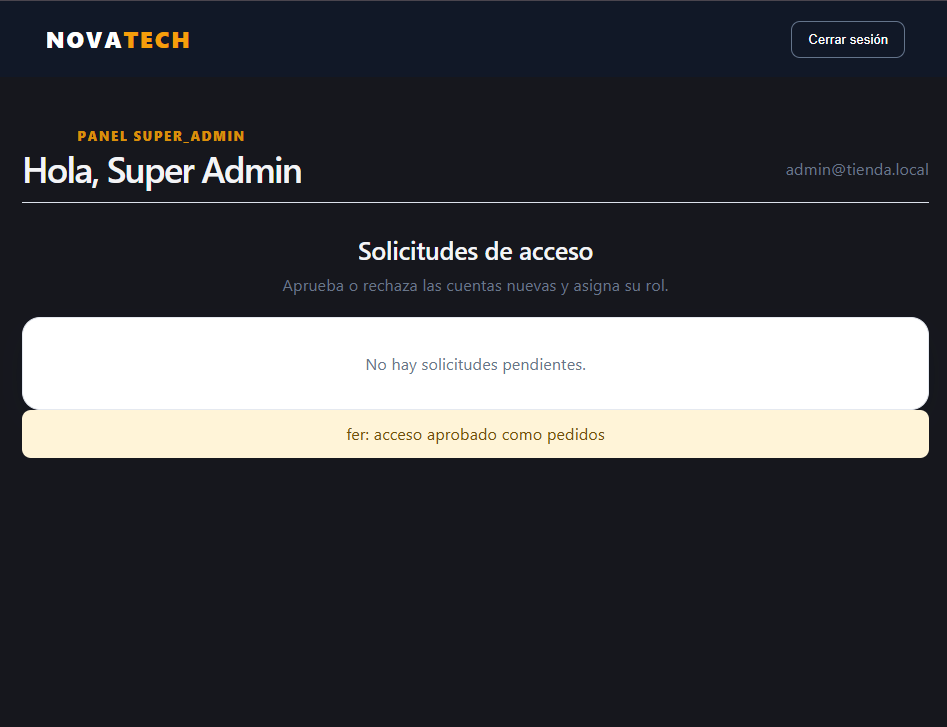
\includegraphics[width=.84\textwidth]{imagenes/04-aprobacion.png}
\caption{La interfaz confirma el acceso aprobado como Pedidos.}
\end{figure}

\clearpage
\begin{figure}[H]\centering
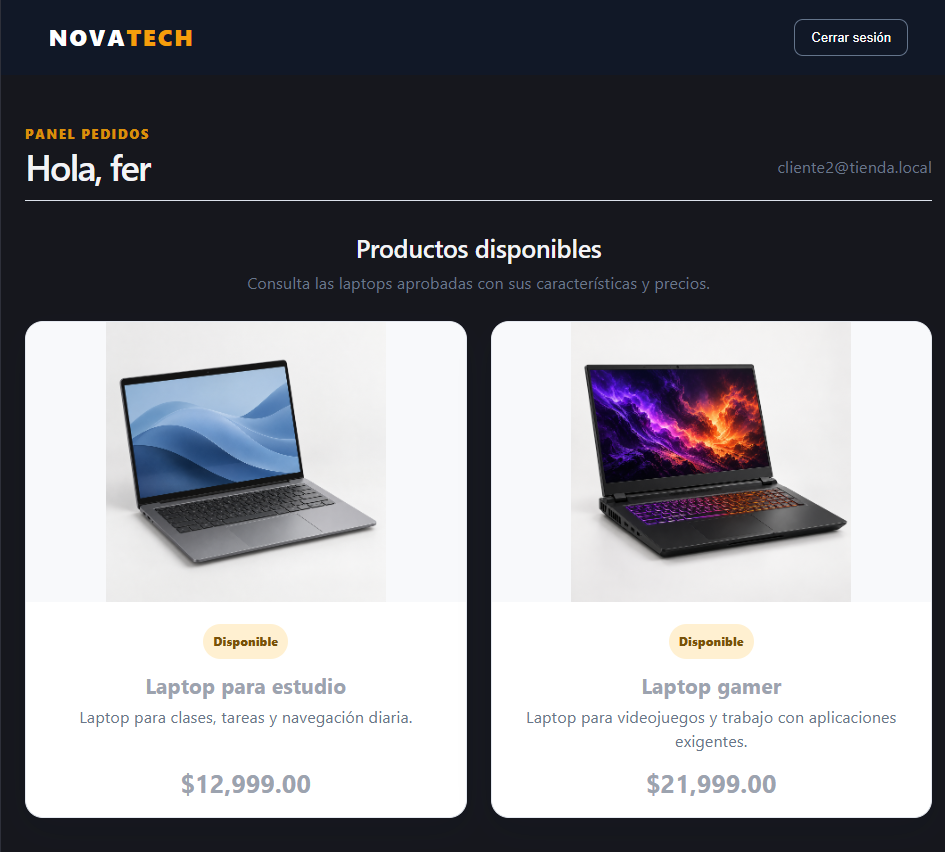
\includegraphics[width=.90\textwidth]{imagenes/05-catalogo.png}
\caption{La cuenta aprobada consulta las dos laptops con imágenes, descripciones y precios.}
\end{figure}

\section{Guía breve para iniciar en WSL}
Con PostgreSQL disponible y la base \texttt{ventas\_taller3} configurada, abrir dos terminales de Ubuntu. En la primera, entrar a \texttt{/mnt/c/proyecto-ventas/backend} e iniciar el servidor con el comando definido en \texttt{backend/package.json}. En la segunda, ejecutar:
\begin{verbatim}
cd /mnt/c/proyecto-ventas/frontend
npm install
npm run dev
\end{verbatim}
Abrir en Windows la dirección \texttt{Local:} que muestre Vite (en las pruebas fue \texttt{http://localhost:5173/}). El servicio del frontend apunta al backend en \texttt{http://localhost:4000/api}. Las dependencias del backend se instalan con \texttt{npm install} desde su carpeta; sus variables locales de base de datos deben configurarse en el equipo sin publicarlas.

\section{Repositorio y archivo de Overleaf}
La raíz del repositorio debe contener las carpetas \texttt{backend/}, \texttt{frontend/} y \texttt{documentacion/}. Dentro de \texttt{documentacion/}, subir este \texttt{main.tex} junto con \texttt{imagenes/} y el PDF compilado. Para Overleaf, crear un proyecto en blanco, subir \texttt{main.tex} y la carpeta \texttt{imagenes/}, y compilar con pdfLaTeX. El archivo \texttt{main.tex} permite editar el contenido sin rehacer el documento.

Antes de publicar en GitHub, revisar \texttt{git status} y excluir \texttt{node\_modules/}, \texttt{.env}, claves y archivos de compilación. Agregar un \texttt{.env.example} con nombres de variables y valores ficticios, si el backend requiere configuración. No hay URL de repositorio confirmada en esta documentación; se añade cuando el repositorio se haya creado y publicado.

\section{Pendientes de la actividad completa}
Quedan por documentar e implementar, según la consigna general, los CRUD de Usuario, Producto y Pedido; las interfaces de Admin y Productos; el captcha de diez imágenes; y el flujo de aprobación de registro y venta de productos. La pantalla de Pedidos de esta etapa ofrece consulta del catálogo. Esta lista permite presentar con claridad el avance real del sábado.

\end{document}
